\bta{功和功率}


\begin{enumerate}[leftmargin=0em]
\renewcommand{\labelenumi}{\arabic{enumi}.}
% A(\Alph) a(\alph) I(\Roman) i(\roman) 1(\arabic)
%设定全局标号series=example	%引用全局变量resume=example
%[topsep=-0.3em,parsep=-0.3em,itemsep=-0.3em,partopsep=-0.3em]
%可使用leftmargin调整列表环境左边的空白长度 [leftmargin=0em]
\item
\exwhere{$ 2018 $年海南卷}
某大瀑布的平均水流量为$ 5900\ m^{3}/s $,水的落差为$ 50\ m $。已知水的密度为$ 1.00 \times \ kg/m^{3} $。在大瀑布水流下落过程中,重力做功的平均功率约为 \xzanswer{D} 



\fourchoices
{$ 3 \times 10 ^ { 6 } \ \mathrm { W } $}
{$ 3 \times 10 ^ { 7 } \ \mathrm { W } $}
{$ 3 \times 10 ^ { 8 } \ \mathrm { W } $}
{$ 3 \times 10 ^ { 9 } \ \mathrm { W } $}




\item 
\exwhere{$ 2015 $年上海卷}
如图,汽车在平直路面上匀速运动,用跨过光滑定滑轮的轻绳牵引轮船,汽车与滑轮间的绳保持水平。当牵引轮船的绳与水平方向成$ \theta $角时,轮船速度为$ v $,绳的拉力对船做功的功率为$ P $,此时绳对船的拉力为 \tk{$\frac { P } { v \cos \theta }$} 
。若汽车还受到恒定阻力$ f $,则汽车发动机的输出功率为 \tk{$f v \cos \theta + P$} 
。
\begin{figure}[h!]
\centering
\includesvg[width=0.23\linewidth]{picture/svg/732}
\end{figure}


\item
\exwhere{$ 2015 $年理综新课标$ \lmd{2} $卷}
一汽车在平直公路上行驶。从某时刻开始计时,发动机的功率$ P $随时间$ t $的变化如图所示。假定汽车所受阻力的大小$ f $恒定不变。下列描述该汽车的速度$ v $随时间$ t $变化的图像中,可能正确的是 \xzanswer{A} 

\begin{figure}[h!]
\centering
\includesvg[width=0.18\linewidth]{picture/svg/733} \qquad 
 \includesvg[width=0.73\linewidth]{picture/svg/734} 
\end{figure}


\item
\exwhere{$ 2011 $年物理江苏卷}
如图所示,演员正在进行杂技表演。由图可估算出他将一只鸡蛋抛出的过程中对鸡蛋所做的功最接近于 \xzanswer{A} 
\begin{figure}[h!]
\centering
\includesvg[width=0.16\linewidth]{picture/svg/735}
\end{figure}

\fourchoices
{$ 0.3\ J $ }
{$ 3\ J $}
{$ 30\ J $ }
{$ 300\ J $}




\item 
\exwhere{$ 2015 $年海南卷}
假设摩托艇受到的阻力的大小正比于它的速率。如果摩托艇发动机的输出功率变为原来的$ 2 $倍,则摩托艇的最大速率变为原来的 \xzanswer{D} 

\fourchoices
{$ 4 $倍 }
{$ 2 $倍}
{$\sqrt{3}$倍}
{$\sqrt{2}$倍}



\item
\exwhere{$ 2012 $年物理江苏卷}
如图所示,细线的一端固定于$ O $点,另一端系一小球. 在水平拉力作用下,小球以恒定速率在竖直平面内由$ A $点运动到$ B $点. 在此过程中拉力的瞬时功率变化情况是 \xzanswer{A} 
\begin{figure}[h!]
\centering
\includesvg[width=0.23\linewidth]{picture/svg/736}
\end{figure}



\fourchoices
{逐渐增大}
{逐渐减小}
{先增大,后减小}
{先减小,后增大}




\item 
\exwhere{$ 2012 $年理综四川卷}
如图所示,劲度系数为$ k $的轻弹簧的一端固定在墙上,另一端与置于水平面上质量为$ m $的物体接触(未连接),弹簧水平且无形变。用水平力,缓慢推动物体,在弹性限度内弹簧长度被压缩了$ x_{0} $,此时物体静止。撤去$ F $后,物体开始向左运动,运动的最大距离为$ 4x_0 $。物体与水平面间的动摩擦因数为$ \mu $,重力加速度为$ g $。则 \xzanswer{BD} 
\begin{figure}[h!]
\centering
\includesvg[width=0.23\linewidth]{picture/svg/737}
\end{figure}

\fourchoices
{撤去$ F $后,物体先做匀加速运动,再做匀减速运动}
{撤去$ F $后,物体刚运动时的加速度大小为$\frac { k x _ { 0 } } { m } - \mu g$}
{物体做匀减速运动的时间为$2 \sqrt{ \frac { x _ { 0 } } { \mu g } }$}
{物体开始向左运动到速度最大的过程中克服摩擦力做的功为$\mu m g \left( x _ { 0 } - \frac { \mu m g } { k } \right)$}


\item
\exwhere{$ 2012 $年理综福建卷}
如图,表面光滑的固定斜面顶端安装一定滑轮,小物块$ A $、$ B $用轻绳连接并跨过滑轮(不计滑轮的质量和摩擦)。初始时刻,$ A $、$ B $处于同一高度并恰好静止状态。剪断轻绳后$ A $下落、$ B $沿斜面下滑,则从剪断轻绳到物块着地,两物块 \xzanswer{D} 
\begin{figure}[h!]
\centering
\includesvg[width=0.23\linewidth]{picture/svg/738}
\end{figure}

\fourchoices
{速率的变化量不同}
{机械能的变化量不同}
{重力势能的变化量相同}
{重力做功的平均功率相同}




\item 
$ 2018 $年江苏卷$ 7 $.如图所示,轻质弹簧一端固定,另一端连接一小物块,$ O $点为弹簧在原长时物块的位置.物块由$ A $点静止释放,沿粗糙程度相同的水平面向右运动,最远到达$ B $点。在从$ A $到$ B $的过程中,物块 \xzanswer{AD} 
\begin{figure}[h!]
\centering
\includesvg[width=0.23\linewidth]{picture/svg/739}
\end{figure}

\fourchoices
{加速度先减小后增大}
{经过$ O $点时的速度最大}
{所受弹簧弹力始终做正功}
{所受弹簧弹力做的功等于克服摩擦力做的功}


\item
\exwhere{$ 2018 $年天津卷}
我国自行研制、具有完全自主知识产权的新一代大型喷气式客机$ C919 $首飞成功后,拉开了全面试验试飞的新征程,假设飞机在水平跑道上的滑跑是初速度为零的匀加速直线运动,当位移$ x=1.6 \times 10^3 $ $ m $时才能达到起飞所要求的速度$ v=80 $ $ m/s $,已知飞机质量$ m=7.0 \times 10^4 $ $ kg $,滑跑时受到的阻力为自身重力的$ 0.1 $倍,重力加速度取$ g=10\ m/s^{2} $,求飞机滑跑过程中:

\begin{enumerate}
\renewcommand{\labelenumi}{\arabic{enumi}.}
% A(\Alph) a(\alph) I(\Roman) i(\roman) 1(\arabic)
%设定全局标号series=example	%引用全局变量resume=example
%[topsep=-0.3em,parsep=-0.3em,itemsep=-0.3em,partopsep=-0.3em]
%可使用leftmargin调整列表环境左边的空白长度 [leftmargin=0em]
\item
加速度$ a $的大小;
\item 
牵引力的平均功率$ P $。



\end{enumerate}
\begin{figure}[h!]
\flushright 
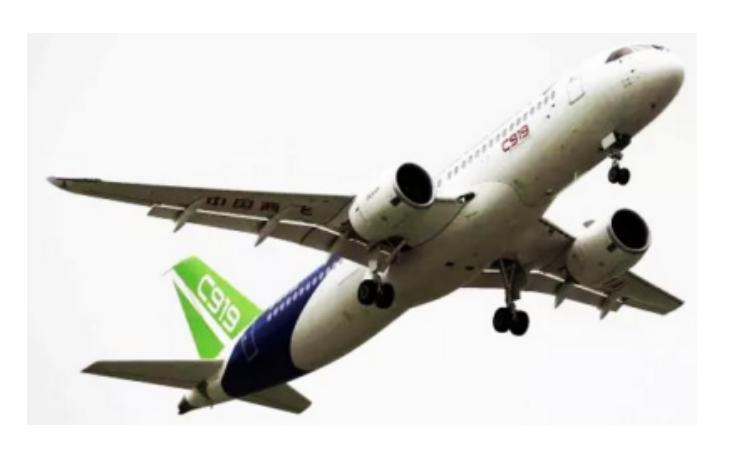
\includegraphics[width=0.3\linewidth]{screenshot015}
\end{figure}

\banswer{
\begin{enumerate}
\renewcommand{\labelenumi}{\arabic{enumi}.}
% A(\Alph) a(\alph) I(\Roman) i(\roman) 1(\arabic)
%设定全局标号series=example	%引用全局变量resume=example
%[topsep=-0.3em,parsep=-0.3em,itemsep=-0.3em,partopsep=-0.3em]
%可使用leftmargin调整列表环境左边的空白长度 [leftmargin=0em]
\item
$ a=2\ m/s^{2} $
\item 
$ P=8.4 \times 10^{6} \ W $

\end{enumerate}


}




\item 
\exwhere{$ 2018 $年浙江卷($ 4 $月选考)}
如图所示,一根绳的两端分别固定在两座猴山的$ A $、$ B $处,$ A $、$ B $两点水平距离为$ 16 \ m $,竖直距离为$ 2 \ m $,$ A $、$ B $间绳长为$ 20 \ m $。质量为$ 10 \ kg $的猴子抓住套在绳子上的滑环从$ A $处滑到$ B $处。以$ A $点所在水平面为参考平面,猴子在滑行过程中重力势能最小值约为(绳处于拉直状态) \xzanswer{B} 
\begin{figure}[h!]
\centering
\includesvg[width=0.23\linewidth]{picture/svg/740}
\end{figure}

\fourchoices
{$ -1.2 \times 10^3 $ $ J $}
{$ -7.5 \times 10^2 $ $ J $}
{$ -6.0 \times 10^2 $ $ J $}
{$ -2.0 \times 10^2 $ $ J $}

\item 
\exwhere{$ 2012 $年物理上海卷}
质量相等的均质柔软细绳$ A $、$ B $平放于水平地面,绳$ A $较长。分别捏住两绳中点缓慢提起,直至全部离开地面,两绳中点被提升的高度分别为$ h_{A} $、$ h_{B} $,上述过程中克服重力做功分别为$ W_A $、$ W_B $。若 \xzanswer{B} 


\fourchoices
{$ h_{A} = h_{B} $,则一定有$ W_A=W_B $}
{$ h_{A} > h_{B} $,则可能有$ W_A<W_B $}
{$ h_{A} < h_{B} $,则可能有$ W_A=W_B $}
{$ h_{A} > h_{B} $,则一定有$ W_A>W_B $}


\item 
\exwhere{$ 2014 $年理综重庆卷}
某车以相同功率在两种不同的水平路面上行驶,受到的阻力分别为车重的$ k_{1} $和$ k_{2} $倍,最大速率分别为$ v_{1} $和$ v_{2} $,则 \xzanswer{B} 

\fourchoices
{$ v _ { 2 } = k _ { 1 } v _ { 1 } $}
{$ v _ { 2 } = \frac { k _ { 1 } } { k _ { 2 } } v _ { 1 } $}
{$ v _ { 2 } = \frac { k _ { 2 } } { k _ { 1 } } v _ { 1 } $}
{$ v _ { 2 } = k _ { 2 } v _ { 1 } $}




\item 
\exwhere{$ 2011 $年海南卷}
一质量为$ 1 \ kg $的质点静止于光滑水平面上,从$ t=0 $时起,第$ 1 $秒内受到$ 2 \ N $的水平外力作用,第$ 2 $秒内受到同方向的$ 1 \ N $的外力作用。下列判断正确的是 \xzanswer{CD} 

\fourchoices
{$ 0 \sim 2s $内外力的平均功率是$ 9/4W $}
{第$ 2 $秒内外力所做的功是$ 5/4J $}
{第$ 2 $秒末外力的瞬时功率最大}
{第$ 1 $秒内与第$ 2 $秒内质点动能增加量的比值是$ 4/5 $}




\item 
\exwhere{$ 2017 $年新课标$ \lmd{2} $卷}
如图,一光滑大圆环固定在桌面上,环面位于竖直平面内,在大圆环上套着一个小环,小环由大圆环的最高点从静止开始下滑,在小环下滑的过程中,大圆环对它的作用力 \xzanswer{A} 

\begin{minipage}[h!]{0.7\linewidth}
\vspace{0.3em}
\fourchoices
{一直不做功}
{一直做正功}
{始终指向大圆环圆心}
{始终背离大圆环圆心}
\vspace{0.3em}
\end{minipage}
\hfill
\begin{minipage}[h!]{0.3\linewidth}
\flushright
\vspace{0.3em}
\includesvg[width=0.5\linewidth]{picture/svg/741}
\vspace{0.3em}
\end{minipage}



\item 
\exwhere{$ 2017 $年海南卷}
将一小球竖直向上抛出,小球在运动过程中所受到的空气阻力不可忽略。$ a $为小球运动轨迹上的一点,小球上升和下降经过$ a $点时的动能分别为$ E_{k} 1 $和$ E_{k} 2 $。从抛出开始到小球第一次经过$ a $点时重力所做的功为$ W_{1} $,从抛出开始到小球第二次经过$ a $点时重力所做的功为$ W_{2} $。下列选项正确的是 \xzanswer{B} 

\fourchoices
{$ E_{k1} = E_{k2} $,$ W_1=W_2 $ }
{$ E_{k1} > E_{k2} $,$ W_1=W_2 $}
{$ E_{k1} < E_{k2} $,$ W_1<W_2 $ }
{$ E_{k1} > E_{k2} $,$ W_1<W_2 $}



\item
\exwhere{$ 2014 $年理综新课标\lmd{2}卷}
一物体静止在粗糙水平地面上,现用一大小为$ F_{1} $的水平拉力拉动物体,经过一段时间后其速度变为$ v $,若将水平拉力的大小改为$ F_{2} $,物体从静止开始经过同样的时间后速度变为$ 2v $,对于上述两个过程,用$ W_{F1} $、$ W_{F2} $分别表示拉力$ F_{1} $、$ F_{2} $所做的功,$ W_{f1} $、$ W_{f2} $分别表示前后两次克服摩擦力所做的功,则 \xzanswer{C} 

\fourchoices
{$ W_{F2}>4W_{F1} $, $ W_{f2}>2W_{f1} $}
{$ W_{F2}>4W_{F1} $,$ W_{f2}=2W_{f1} $}
{$ W_{F2}<4W_{F1} $,$ W_{f2}=2W_{f1} $,}
{$ W_{F2}<4W_{F1} $,$ W_{f2}<2W_{f1} $}




\item 
\exwhere{$ 2012 $年物理上海卷}
位于水平面上的物体在水平恒力$ F_{1} $作用下,做速度为$ v_{1} $的匀速运动;若作用力变为斜向上的恒力$ F_{2} $,物体做速度为$ v_{2} $的匀速运动,且$ F_{1} $与$ F_{2} $功率相同。则可能有 \xzanswer{BD} 
\begin{figure}[h!]
\centering
\includesvg[width=0.3\linewidth]{picture/svg/742}
\end{figure}


\fourchoices
{$ F_2=F_1 $,$ v_{1} > v_{2} $ }
{$ F_2=F_1 $,$ v_{1} < v_{2} $}
{$ F_2>F_1 $,$ v_{1} > v_{2} $}
{$ F_2<F_1 $,$ v_{1} < v_{2} $}




\item 
\exwhere{$ 2011 $年理综四川卷}
如图是“神舟”系列航天飞船返回舱返回地面的示意图,假定其过程可简化为:打开降落伞一段时间后,整个装置匀速下降,为确保安全着陆,需点燃返回舱的缓冲火箭,在火箭喷气过程中返回舱做减速直线运动,则 \xzanswer{A} 
\begin{figure}[h!]
\centering
\includesvg[width=0.23\linewidth]{picture/svg/743}
\end{figure}

\fourchoices
{火箭开始喷气瞬间伞绳对返回舱的拉力变小}
{返回舱在喷气过程中减速的主要原因是空气阻力}
{返回舱在喷气过程中所受合外力可能做正功}
{返回舱在喷气过程中处于失重状态}


\item
\exwhere{$ 2011 $年上海卷}
如图,一长为$ L $的轻杆一端固定在光滑铰链上,另一端固定一质量为$ m $的小球。一水平向右的拉力作用于杆的中点,使杆以角速度$ \omega $匀速转动,当杆与水平方向成$ 60 ^{ \circ } $时,拉力的功率为 \xzanswer{C} 
\begin{figure}[h!]
\centering
\includesvg[width=0.23\linewidth]{picture/svg/744}
\end{figure}

\fourchoices
{$ mgL \omega $}
{$ \frac{\sqrt{3}}{2} mgL \omega $}
{$ \frac{ 1 }{ 2 } mgL \omega $}
{$ \frac{\sqrt{3}}{6} mgL \omega $}


\item 
\exwhere{$ 2015 $年理综浙江卷}
我国科学家正在研制航母舰载机使用的电磁弹射器。舰载机总质量为$ 3.0 \times 10^4 \ kg $,设起飞过程中发动机的推力恒为$ 1.0 \times 10^5 \ N $;弹射器有效作用长度为$ 100 \ m $,推力恒定。要求舰载机在水平弹射结束时速度大小达到$ 80 \ m/s $,弹射过程中舰载机所受总推力为弹射器和发动机推力之和,假设所受阻力为总推力的$ 20 \% $,则 \xzanswer{ABD} 

\fourchoices
{弹射器的推力大小为$ 1.1 \times 10^6 \ N $}
{弹射器对舰载机所做的功为$ 1.1 \times 10^8 \ J $}
{弹射器对舰载机做功的平均功率为$ 8.8 \times 10^7 \ W $}
{舰载机在弹射过程中的加速度大小为$ 32 \ m/s^{2} $}





\newpage
\item
\exwhere{$ 2012 $年理综重庆卷}
如图所示为一种摆式摩擦因数测量仪,可测量轮胎与地面间动摩擦因数,其中主要部件有:底部固定有轮胎橡胶片的摆锤和连接摆锤的轻质细杆。摆锤的质量为$ m $,细杆可绕轴$ O $在竖直平面内自由转动,摆锤重心到$ O $点的距离为$ L $ 。测量时,测量仪固定于水平地面,将摆锤从与$ O $等高的位置由静止释放。摆锤到最低点附近时,橡胶片紧压地面擦过一小段距离$ s(s<<L) $,之后继续摆动至与坚直方向成$ \theta $角的最高位置。若摆锤对地面的压力可视为大小为$ F $的恒力,重力加速度为$ g $,求:

\begin{enumerate}
\renewcommand{\labelenumi}{\arabic{enumi}.}
% A(\Alph) a(\alph) I(\Roman) i(\roman) 1(\arabic)
%设定全局标号series=example	%引用全局变量resume=example
%[topsep=-0.3em,parsep=-0.3em,itemsep=-0.3em,partopsep=-0.3em]
%可使用leftmargin调整列表环境左边的空白长度 [leftmargin=0em]
\item
摆锤在上述过程中损失的机械能;
\item 
在上述过程中摩擦力对摆锤所做的功;
\item 
橡胶片与地面间的动摩擦因数.



\end{enumerate}
\begin{figure}[h!]
\flushright
\includesvg[width=0.28\linewidth]{picture/svg/745}
\end{figure}

\banswer{
\begin{enumerate}
\renewcommand{\labelenumi}{\arabic{enumi}.}
% A(\Alph) a(\alph) I(\Roman) i(\roman) 1(\arabic)
%设定全局标号series=example	%引用全局变量resume=example
%[topsep=-0.3em,parsep=-0.3em,itemsep=-0.3em,partopsep=-0.3em]
%可使用leftmargin调整列表环境左边的空白长度 [leftmargin=0em]
\item
损失的机械能$\Delta E = m g L \cos \theta$
\item 
摩擦力做的功$W _ { f } = - m g L \cos \theta$
\item 
动摩擦因数$\mu = m g L \cos \theta / F S$



\end{enumerate}


}






\item
\exwhere{$ 2016 $年海南卷}
水平地面上有质量分别为$ m $和$ 4 \ m $的物$ A $和$ B $,两者与地面的动摩擦因数均为$ \mu $。细绳的一端固定,另一端跨过轻质动滑轮与$ A $相连,动滑轮与$ B $相连,如图所示。初始时,绳出于水平拉直状态。若物块$ A $在水平向右的恒力$ F $作用下向右移动了距离$ s $,重力加速度大小为$ g $。求:

\begin{enumerate}
\renewcommand{\labelenumi}{\arabic{enumi}.}
% A(\Alph) a(\alph) I(\Roman) i(\roman) 1(\arabic)
%设定全局标号series=example	%引用全局变量resume=example
%[topsep=-0.3em,parsep=-0.3em,itemsep=-0.3em,partopsep=-0.3em]
%可使用leftmargin调整列表环境左边的空白长度 [leftmargin=0em]
\item
物块$ B $克服摩擦力所做的功;
\item 
物块$ A $、$ B $的加速度大小。




\end{enumerate}
\begin{figure}[h!]
\flushright
\includesvg[width=0.3\linewidth]{picture/svg/746}
\end{figure}



\banswer{
\begin{enumerate}
\renewcommand{\labelenumi}{\arabic{enumi}.}
% A(\Alph) a(\alph) I(\Roman) i(\roman) 1(\arabic)
%设定全局标号series=example	%引用全局变量resume=example
%[topsep=-0.3em,parsep=-0.3em,itemsep=-0.3em,partopsep=-0.3em]
%可使用leftmargin调整列表环境左边的空白长度 [leftmargin=0em]
\item
$2 \mu m g s$
\item 
$a _ { \mathrm { A } } = \frac { F - 3 \mu m g } { 2 m } , \quad a _ { \mathrm { B } } = \frac { F - 3 \mu m g } { 4 m }$

\end{enumerate}


}








\end{enumerate}

